\section{Chiang Mai}

Date: 26/06/2008

\begin{multicols}{2}

Amis du voyage, Bonjour !!!

Nous attaquons une série d'articles évolutifs car certaines photos que je vais récupérer d'autres gens viendrons s'ajouter aux miennes, au fil du temps. Je voyage maintenant et encore pour quelques jours avec Arnaud.

Aujourd'hui nous allons parler de Chiang Mai, ville du nord de la Thaïlande dans laquelle je suis resté 5 jours. En fait, plutôt que de vous parler de Chiang Mai, je vous propose de parler des environs de Chiang Mai, car comme à mon habitude maintenant je ne suis pas trop resté dans les murs de la ville mais j'ai préféré louer une motor bike pour aller é la campagne, voir des gens que le tourisme ne touche pas... et que l'anglais ne touche pas non plus, d'où pas mal de difficultés, et de gêne.

Nous sommes allés nous ballader avec Arnaud, jeune Français comme moi qui fait un voyage en Asie de deux mois.

Direction le nord, où nous suivons une route de montagne sur une trentaine de kilomètres. Puis un autre jour, nous descendons au Sud, environs 80km pour aller dans un parc national. Nous nous arrêtons le midi dans un petit warung (genre snack pas cher) pour manger un riz frit ou autre fried noodles et nous tombons sur deux mecs, bien saouls, la bouteille de whiskey à moitié vide sur la table. Ils nous invitent à venir nous joindre à leur table. Vu qu'on est pas du genre à dire non, on y va. Et là on s'aperçoit vite que c'était un traquenard, en fait on est la curiosité du moment et d'autres mecs arrivent, on boit tous, on se fait offrir une soupe aux crevettes, on boit, on prend des photos, on boit... Bon c'est pas tous ça mais le temps est très gris, saisons des pluies oblige, on a décidé d'aller voir le parc, et de faire les 80km pour rentrer après, va falloir y aller molo sur la picole !!!

\hspace*{-0.65cm}
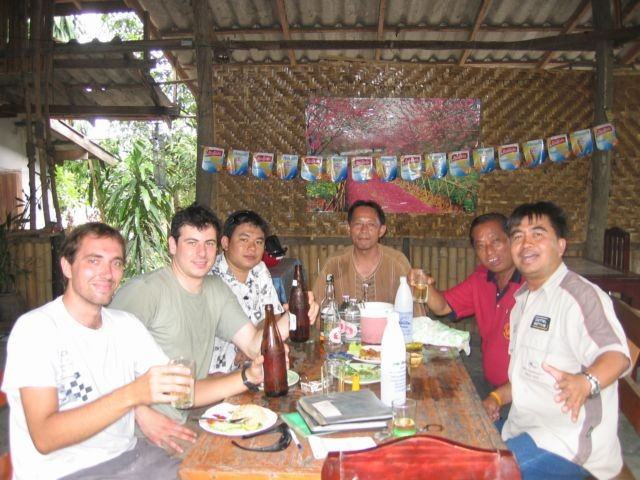
\includegraphics[width=4.8cm]{articles/Chiang-mai/1214286196a5oS.jpg}
Bah c'est du propre, tiens !

\hspace*{-0.65cm}
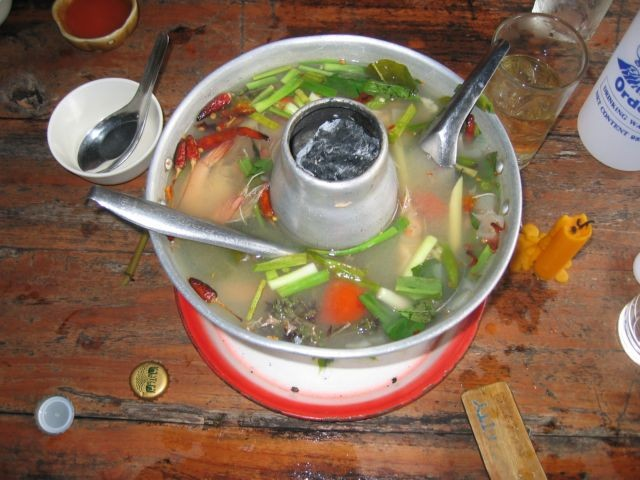
\includegraphics[width=4.8cm]{articles/Chiang-mai/1214286184dsFU.jpg}
Soupe de piment.

Mon passage a Chiang Mai n'aurait pas été le même sans la Julie's Guest House, c'est pourquoi je me dois d'en dire quelques mots. Le concept : les chambre les moins chères que j'ai vues en Thailande, les boissons à volonté (il suffit de marquer ses consommations sur un carnet dédié et on paie a la fin), plusieurs espace de détente où il est très facile de rester une journée entière à discuter avec d'autres voyageurs, jouer au billiard... ou regarder l'euro 2008 à 2h du matin.

\hspace*{-0.65cm}
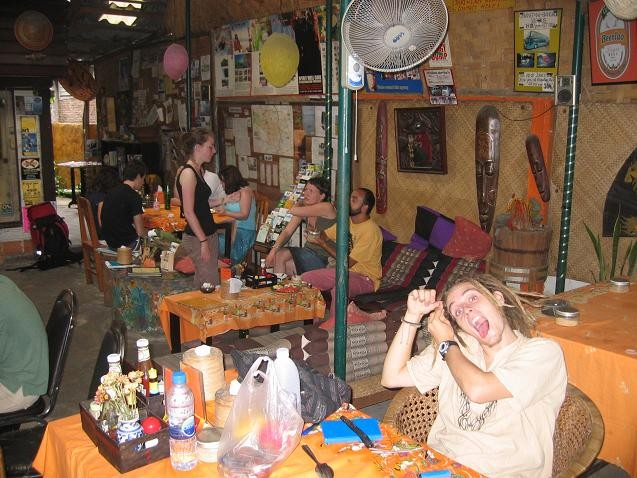
\includegraphics[width=4.8cm]{articles/Chiang-mai/1214471834JD3r.jpg}
La Julie's guest house, au top !

Pour terminer, et par ce que j'ai envie de vous poser une question qui n'a rien à voir, voici une devinette : Devinez le nom de ce très bon fruit.

\hspace*{-0.65cm}
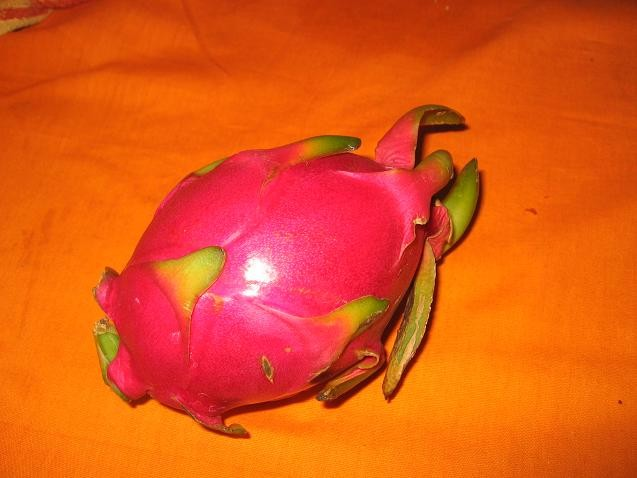
\includegraphics[width=4.8cm]{articles/Chiang-mai/1214471825EGhM.jpg}
Mais quelle est ce fruit ?

\end{multicols}

\bigskip
\textbf{\textsc{Commentaires}}

\medskip
Titou a écrit le 26 juin 2008 :
\begin{displayquote}
eheh ! Encore de jolies photos que voila ! Comme tu le vois je n'ai pas pu attendre ce soir ni demain pour faire ma lecture !
Ralala ça donne envie, tu me raconteras tout ça en détails devant une bonne bière à ton retour !
A plus ti dud !
ps : pour le fruit j'ai pas trouvé alors c'est pour ça que j'ai rien dit :p
\end{displayquote}

\medskip
Chachou a écrit le 27 juin 2008 :
\begin{displayquote}
Coucou,
Toujours des photos qui font envie (quoi que la soupe de crevettes, pas plus envie que ça...).
On gagne quoi si on répond bien à la devinette?
Fruit du dragon ou pitaya rose à chair blanche
Bonne continuation
Bisous ;-)
\end{displayquote}

\medskip
Etienne a écrit le 27 juin 2008 :
\begin{displayquote}
Ok Chachou, bien joue c'est un fruit du dragon. Je t'aurais bien dit que tu en gagnes un mais il risquerais de ne plus etre bon apres 10 jours a Bali. Et comme ton mec ne veux pas que je te fasse de bisous, ben du coup je vais essayer de trouver une autre idee.
\end{displayquote}


